\documentclass{beamer} 
\usetheme{default} 
\setbeamercovered{transparent}

%\useoutertheme{umbcfootline} 
\setbeamertemplate{background canvas}[vertical shading][bottom=red!20,top=yellow!30] 


\usepackage[spanish]{babel}
%\usepackage[latin1]{inputenc}
\usepackage[utf8x]{inputenc}
\usepackage{multicol}


\title{JDBC}

\author{Manuel J. Molino Milla \and Luis Molina Garzón}

\date{\today} %

\institute{IES Virgen del Carmen \and Departamento de Informática}




%\beamerdefaultoverlayspecification{<+->}

\begin{document}


\begin{frame}
  \titlepage
\end{frame}

\begin{frame}
    \frametitle{Logo}
\begin{figure}
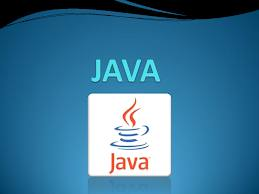
\includegraphics[scale=1]{imagenes/logo.jpeg} 
\caption{Logo Java}
\end{figure}
\end{frame}

\begin{frame}
  \frametitle{Contenido}
 \tableofcontents[pausesections]
\end{frame}



\section{Introduccion}
\begin{frame}[fragile]
\frametitle{Introducción a JDBC}
\begin{scriptsize}
\begin{itemize}[<+->]
\item El API \alert{JDBC} permite el acceso a datos tabulados, sobre todo a aquellos que se almacenan en \emph{base de datos relacionales}.
\item JDBC permite:
\begin{enumerate}
\item Conectar a la fuente de datos, como es la base de datos.
\item Enviar consultas y realizar actualizaciones sobre la base de datos.
\item Recuperar y procesar resultados recibidos de la \emph{BD} en respuesta a la consulta.
\end{enumerate}
\item El siguiente fragmento de código resume un ejemplo de conexión:
\end{itemize}
\end{scriptsize}
\pause
\begin{tiny}
\begin{verbatim}
public void connectToAndQueryDatabase(String username, String password) {

    Connection con = DriverManager.getConnection(
                         "jdbc:myDriver:myDatabase",
                         username,
                         password);

    Statement stmt = con.createStatement();
    ResultSet rs = stmt.executeQuery("SELECT a, b, c FROM Table1");

    while (rs.next()) {
        int x = rs.getInt("a");
        String s = rs.getString("b");
        float f = rs.getFloat("c");
    }
}
\end{verbatim}
\end{tiny}
\end{frame}

\begin{frame}[fragile]
\frametitle{Ejemplo de UPDATE}
\begin{tiny}
\begin{verbatim}
import java.sql.*;

public class UpdateCar {

    public static void UpdateCarNum(int carNo, int empNo)
        throws SQLException {

        Connection con = null;
        PreparedStatement pstmt = null;   
      
        try {
            con = DriverManager.getConnection(
                      "jdbc:default:connection");

            pstmt = con.prepareStatement(
                        "UPDATE EMPLOYEES " +
                        "SET CAR_NUMBER = ? " +
                        "WHERE EMPLOYEE_NUMBER = ?");

            pstmt.setInt(1, carNo);
            pstmt.setInt(2, empNo);
            pstmt.executeUpdate();
        }
        finally {
            if (pstmt != null) pstmt.close();
        }
    }
}
\end{verbatim}
\end{tiny}
\end{frame}

\section{Procesando sentencias SQL}
\begin{frame}[fragile]
\frametitle{Procesando sentencias SQL} 
\begin{block}{Establecimiento de la conexion}
Primer hay que establecer la conexión. Se utiliza un objeto del tipo \alert{Connection}
\pause
\begin{scriptsize}
\begin{verbatim}
String url = "jdbc:mysql://localhost/test";
Class.forName ("com.mysql.jdbc.Driver").newInstance ();
Connection conn = DriverManager.getConnection (url, "username", "password");
\end{verbatim}
\end{scriptsize}
\end{block} 
\pause
\begin{block}{Creacion de las sentencias}
Se utiliza la interfaz \alert{Statement} y genera objetos de tipo \alert{ResultSet}. Hay tres tipos de \emph{consultas}:
\begin{enumerate}[<+->]
\item \alert{Statement} implementa sentencias simples SQL sin parámetros.
\item \alert{PreparedStatement} usada para precompilar sentencias que pueden contener parámetros.
\item \alert{CallableStatement} extiendo de \emph{PreparedStatement} usados tanto en la entrada como salida de datos.
\end{enumerate}
\end{block}
\end{frame}

\begin{frame}[fragile]
\frametitle{Procesando sentencias SQL} 
\begin{tiny}
\begin{block}{Ejecucion de consultas}
Se usa un métodos \alert{execute} desde un objeto \emph{Statement}:
\begin{enumerate}[<+->]
\item \alert{execute} devuelve \emph{true} si se devuelve un objeto de tipo \emph{ResultSet}
\item \alert{executeQuery} devuelve un objeto de tipo \emph{ResultSet}.
\item \alert{executeUpdate} usado para sentencias INSERT, DELETE, o UPDATE
\item Ejemplo: \emph{ResultSet rs = stmt.executeQuery(query);}
\end{enumerate}
\end{block} 
\pause
\begin{block}{Procesando objetos ResultSet}
\begin{verbatim}
try {
    stmt = con.createStatement();
    ResultSet rs = stmt.executeQuery(query);
    while (rs.next()) {
        String coffeeName = rs.getString("COF_NAME");
        int supplierID = rs.getInt("SUP_ID");
        float price = rs.getFloat("PRICE");
        int sales = rs.getInt("SALES");
        int total = rs.getInt("TOTAL");
        System.out.println(coffeeName + "\t" + supplierID +
                           "\t" + price + "\t" + sales +
                           "\t" + total);
    }
}
// ...
\end{verbatim}
\end{block}
\end{tiny}
\end{frame}


\begin{frame}[fragile]
\frametitle{Procesando sentencias SQL} 
\begin{block}{Cerrando la conexion}
\begin{itemize}[<+->]
\item Cuando dejemos de usar el objeto \emph{Statement} debemos llamar al método \alert{Statement.close}, de esta manera todos los objetos \emph{ResultSet} son cerrados.
\item Ejemplo:
\end{itemize}
\pause
\begin{verbatim}
      } finally {
           if (stmt != null) { stmt.close(); }
      }
\end{verbatim}
\end{block}
\end{frame}


\section{DriverManager}
\begin{frame}[fragile]
\frametitle{DriverManager}
\begin{itemize}[<+->]
\item La clase \emph{DriverManager} se encarga del manejo de la conexión con la BD.
\item Contiene métodos para trabajar con un conjunto de controladores JDBC.
\item Todos conllevan cargar el driver que se suministra como una librería \emph{jar}
\item Ejemplo en mysql:
\end{itemize}
\pause
\begin{tiny}
\begin{verbatim}
import java.sql.Connection;
import java.sql.DriverManager;
import java.sql.SQLException;

Connection conn = null;
...
try {
    conn =
       DriverManager.getConnection("jdbc:mysql://localhost:3306/test?" +
                                   "user=monty&password=greatsqldb");

    // Do something with the Connection

   ...
} catch (SQLException ex) {
    // handle any errors
    System.out.println("SQLException: " + ex.getMessage());
    System.out.println("SQLState: " + ex.getSQLState());
    System.out.println("VendorError: " + ex.getErrorCode());
}
\end{verbatim}
\end{tiny}
\end{frame}


\begin{frame}[fragile]
\frametitle{Driver Sqlite}
\begin{footnotesize}
\begin{verbatim}
import java.sql.*;

public class SQLiteJDBC
{
  public static void main( String args[] )
  {
    Connection c = null;
    try {
      Class.forName("org.sqlite.JDBC");
      c = DriverManager.getConnection("jdbc:sqlite:test.db");
    } catch ( Exception e ) {
      System.err.println( e.getClass().getName() + ": " 
                                     + e.getMessage() );
      System.exit(0);
    }
    System.out.println("Opened database successfully");
  }
}
\end{verbatim}
\end{footnotesize}
\end{frame}



\begin{frame}[fragile]
\frametitle{Driver Oracle}
\begin{tiny}
\begin{verbatim}
// Example Java Program - Oracle Database Connectivity
import java.sql.Connection;
import java.sql.Date;
import java.sql.DriverManager;
import java.sql.ResultSet;
import java.sql.SQLException;
import java.sql.Statement;
public class OracleSample {
    public static final String DBURL = "jdbc:oracle:thin:@localhost:1521:XE";
    public static final String DBUSER = "system";
    public static final String DBPASS = "manager";
    public static void main(String[] args) throws SQLException {
    // Load Oracle JDBC Driver
    DriverManager.registerDriver(new oracle.jdbc.driver.OracleDriver());
    // Connect to Oracle Database
    Connection con = DriverManager.getConnection(DBURL, DBUSER, DBPASS);
    Statement statement = con.createStatement();
    // Execute a SELECT query on Oracle Dummy DUAL Table.
    // Enables us to retrieve values as if querying from a table
       ResultSet rs = statement.executeQuery("SELECT SYSDATE FROM DUAL");
       if (rs.next()) {
           Date currentDate = rs.getDate(1); // get first column returned
           System.out.println("Current Date from Oracle is : "+currentDate);
       }
       rs.close();
    statement.close();
    con.close();
    }
}
\end{verbatim}
\end{tiny}
\end{frame}

\begin{frame}[fragile]
\frametitle{Driver PostgreSQL}
\begin{scriptsize}
\begin{verbatim}
import java.sql.Connection;
import java.sql.DriverManager;

public class PostgreSQLJDBC {
   public static void main(String args[]) {
      Connection c = null;
      try {
         Class.forName("org.postgresql.Driver");
         c = DriverManager
            .getConnection("jdbc:postgresql://localhost:5432/testdb",
            "postgres", "123");
      } catch (Exception e) {
         e.printStackTrace();
         System.err.println(e.getClass().getName()+": "+e.getMessage());
         System.exit(0);
      }
      System.out.println("Opened database successfully");
   }
}
\end{verbatim}
\end{scriptsize}
\end{frame}


\begin{frame}[fragile]
\frametitle{Driver SQL Server}
\begin{tiny}
\begin{verbatim}
    public class JdbcSQLServerDriverUrlExample
{
  public static void main(String[] args)
  {
    Connection connection = null;
    try
    {
      // the sql server driver string
      Class.forName("com.microsoft.sqlserver.jdbc.SQLServerDriver");

      // the sql server url
      String url = "jdbc:microsoft:sqlserver://HOST:1433;DatabaseName=DATABASE";

      // get the sql server database connection
      connection = DriverManager.getConnection(url,"THE_USER", "THE_PASSWORD");

      // now do whatever you want to do with the connection
      // ...

    }
    catch (ClassNotFoundException e)
    {
      e.printStackTrace();
      System.exit(1);
    }
    catch (SQLException e)
    {
      e.printStackTrace();
      System.exit(2);
    }
  }
}
\end{verbatim}
\end{tiny}
\end{frame}


\section{SQLException}
\begin{frame}[fragile]
\frametitle{Manejo de SQLException}
\begin{scriptsize}
Cuando \emph{JDBC} encuentra un error durante la interacción con la BD lanzará una instanica de \alert{SQLException}. Éste objeto contiene la siguiente información:
\begin{itemize}[<+->]
\item Una descripción del error llamando al método \emph{SQLException.getMessage.}
\item Un código de estado con \emph{SQLException.getSQLState.}
\item Un código de error con \emph{ SQLException.getErrorCode.}
\item La causa de la excepción con \emph{SQLException.getCause}
\item Una referencia a la siguiente excepción con \emph{ SQLException.getNextException}
\end{itemize}
\pause
\begin{verbatim}
e.printStackTrace(System.err);
System.err.println("SQLState: " +
       ((SQLException)e).getSQLState());
System.err.println("Error Code: " +
       ((SQLException)e).getErrorCode());
System.err.println("Message: " + e.getMessage());
Throwable t = ex.getCause();
    while(t != null) {
        System.out.println("Cause: " + t);
        t = t.getCause();
    }
\end{verbatim}
\end{scriptsize}
\end{frame}

\section{Resulset}
\begin{frame}[fragile]
\frametitle{Obteniendo valores de ResultSet}
\begin{tiny}
\begin{verbatim}
public static void viewTable(Connection con, String dbName)
    throws SQLException {

    Statement stmt = null;
    String query =
        "select COF_NAME, SUP_ID, PRICE, " +
        "SALES, TOTAL " +
        "from " + dbName + ".COFFEES";

    try {
        stmt = con.createStatement();
        ResultSet rs = stmt.executeQuery(query);
        while (rs.next()) {
            String coffeeName = rs.getString("COF_NAME");
            int supplierID = rs.getInt("SUP_ID");
            float price = rs.getFloat("PRICE");
            int sales = rs.getInt("SALES");
            int total = rs.getInt("TOTAL");
            System.out.println(coffeeName + "\t" + supplierID +
                               "\t" + price + "\t" + sales +
                               "\t" + total);
        }
    } catch (SQLException e ) {
        JDBCTutorialUtilities.printSQLException(e);
    } finally {
        if (stmt != null) { stmt.close(); }
    }
}
\end{verbatim}
\end{tiny}
\end{frame}

\begin{frame}
\frametitle{Correspondencia de tipos}
\begin{figure}
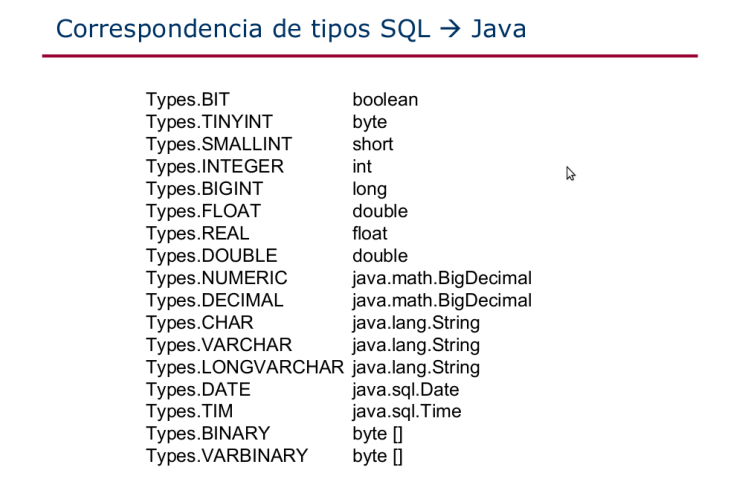
\includegraphics[scale=0.5]{imagenes/correspondencia.png}
\end{figure}
\end{frame}

\begin{frame}[fragile]
\frametitle{Actualizando valores con ResultSet}
\begin{footnotesize}
\begin{verbatim}
Statement stmt = null;
    try {
        stmt = con.createStatement();
        stmt = con.createStatement(ResultSet.TYPE_SCROLL_SENSITIVE,
                   ResultSet.CONCUR_UPDATABLE);
        ResultSet uprs = stmt.executeQuery(
            "SELECT * FROM " + dbName + ".COFFEES");

        while (uprs.next()) {
            float f = uprs.getFloat("PRICE");
            uprs.updateFloat( "PRICE", f * percentage);
            uprs.updateRow();
        }

    } catch (SQLException e ) {
        JDBCTutorialUtilities.printSQLException(e);
    } finally {
        if (stmt != null) { stmt.close(); }
    }
}
\end{verbatim}
\end{footnotesize}
\end{frame}


\begin{frame}[fragile]
\frametitle{Eliminacion de datos}
\begin{footnotesize}
\begin{verbatim}
// Define la conexión
 Connection laConexion = AdministradorDeConexiones.getConnection();       
// Arma la sentencia de eliminación y la ejecuta
 String laEliminacion = "DELETE FROM alumnos WHERE alu_id = 101";
 Statement stmtEliminacion = laConexion.createStatement();
 stmtEliminacion.execute(laEliminacion);       
// Cierra el Statement y la Connection
stmtEliminacion.close();
laConexion.close();       
// Informa que la eliminación ha sido realizada con éxito
System.out.println("La eliminación ha sido realizada con éxito...");
\end{verbatim}
\end{footnotesize}
\end{frame}

\section{Transacciones}
\begin{frame}[fragile]
\frametitle{Transacciones}
\begin{tiny}
\begin{itemize}[<+->]
\item Una transacción es un conjunto de una o mas sentencias que se ejecutan de forma atómica (como solo una), por lo que se ejecutan todas o no se ejecuta ninguna.
\item Cuando se crea con \emph{JDBC} una conexión, esta se crea en modo \alert{auto-commit}, esto significa que cada sentencia SQL individual es tratada como una transacción.
\item La manera que mas de una sentencia puedan ser agrupadas como una única \emph{transacción} es desactivar el \emph{auto-commit} con \alert{con.setAutoCommit(false);}
\end{itemize}
\pause
\begin{verbatim}
public void updateCoffeeSales(HashMap<String, Integer> salesForWeek)
    throws SQLException {

    PreparedStatement updateSales = null;
    PreparedStatement updateTotal = null;
    String updateString =
        "update " + dbName + ".COFFEES " +
        "set SALES = ? where COF_NAME = ?";

    String updateStatement =
        "update " + dbName + ".COFFEES " +
        "set TOTAL = TOTAL + ? " +
        "where COF_NAME = ?";
    try {
        con.setAutoCommit(false);
        updateSales = con.prepareStatement(updateString);
        updateTotal = con.prepareStatement(updateStatement);
        for (Map.Entry<String, Integer> e : salesForWeek.entrySet()) {
            updateSales.setInt(1, e.getValue().intValue());
            updateSales.setString(2, e.getKey());
            updateSales.executeUpdate();
            updateTotal.setInt(1, e.getValue().intValue());
            updateTotal.setString(2, e.getKey());
            updateTotal.executeUpdate();
            con.commit();
        }
\end{verbatim}
\begin{center}
Continua \dots
\end{center}\end{tiny}
\end{frame}



\begin{frame}[fragile]
\frametitle{Transacciones}
\begin{footnotesize}
\begin{verbatim}
   } catch (SQLException e ) {
        JDBCTutorialUtilities.printSQLException(e);
        if (con != null) {
            try {
                System.err.print("Transaction is being rolled back");
                con.rollback();
            } catch(SQLException excep) {
                JDBCTutorialUtilities.printSQLException(excep);
            }
        }
    } finally {
        if (updateSales != null) {
            updateSales.close();
        }
        if (updateTotal != null) {
            updateTotal.close();
        }
        con.setAutoCommit(true);
    }
}
\end{verbatim}
\end{footnotesize}
\end{frame}


\section{Statement}
\begin{frame}[fragile]
\frametitle{Usando Objetos Statement Objects para Batch Updates}
\begin{tiny}
\begin{verbatim}
public void batchUpdate() throws SQLException {
    Statement stmt = null;
    try {
        this.con.setAutoCommit(false);
        stmt = this.con.createStatement();
        stmt.addBatch(
            "INSERT INTO COFFEES " +
            "VALUES('Amaretto', 49, 9.99, 0, 0)");
        stmt.addBatch(
            "INSERT INTO COFFEES " +
            "VALUES('Hazelnut', 49, 9.99, 0, 0)");
        stmt.addBatch(
            "INSERT INTO COFFEES " +
            "VALUES('Amaretto_decaf', 49, " +
            "10.99, 0, 0)");
        stmt.addBatch(
            "INSERT INTO COFFEES " +
            "VALUES('Hazelnut_decaf', 49, " +
            "10.99, 0, 0)");
        int [] updateCounts = stmt.executeBatch();
        this.con.commit();
    } catch(BatchUpdateException b) {
        JDBCTutorialUtilities.printBatchUpdateException(b);
    } catch(SQLException ex) {
        JDBCTutorialUtilities.printSQLException(ex);
    } finally {
        if (stmt != null) { stmt.close(); }
        this.con.setAutoCommit(true);
    }
}
\end{verbatim}
\end{tiny}
\end{frame}

\begin{frame}[fragile]
\frametitle{Usando Prepared Statements}
\begin{tiny}
\begin{verbatim}
public void updateCoffeeSales(HashMap<String, Integer> salesForWeek) throws SQLException {
    PreparedStatement updateSales = null; PreparedStatement updateTotal = null;
    String updateString = "update " + dbName + ".COFFEES " + "set SALES = ?
     where COF_NAME = ?";
    String updateStatement = 
    "update " + dbName + ".COFFEES " +"set TOTAL = TOTAL + ? " + "where COF_NAME = ?";
    try { con.setAutoCommit(false);
        updateSales = con.prepareStatement(updateString);
        updateTotal = con.prepareStatement(updateStatement);
        for (Map.Entry<String, Integer> e : salesForWeek.entrySet()) {
            updateSales.setInt(1, e.getValue().intValue());
            updateSales.setString(2, e.getKey());
            updateSales.executeUpdate();
            updateTotal.setInt(1, e.getValue().intValue());
            updateTotal.setString(2, e.getKey());
            updateTotal.executeUpdate();
            con.commit();
        }
    } catch (SQLException e ) { JDBCTutorialUtilities.printSQLException(e);
        if (con != null) {
            try { System.err.print("Transaction is being rolled back");
                con.rollback();
            } catch(SQLException excep) {
                JDBCTutorialUtilities.printSQLException(excep);
            }
        }
    } finally {
        if (updateSales != null) {
            updateSales.close();
        }
        if (updateTotal != null) {
            updateTotal.close();
        }
        con.setAutoCommit(true);
    }
}
\end{verbatim}
\end{tiny}
\end{frame}

\begin{frame}[fragile]
\frametitle{Creando tablas}
\begin{footnotesize}
\begin{verbatim}
public void createTable() throws SQLException {
    String createString =
        "create table " + dbName +
        ".SUPPLIERS " +
        "(SUP_ID integer NOT NULL, " +
        "SUP_NAME varchar(40) NOT NULL, " +
        "STREET varchar(40) NOT NULL, " +
        "CITY varchar(20) NOT NULL, " +
        "STATE char(2) NOT NULL, " +
        "ZIP char(5), " +
        "PRIMARY KEY (SUP_ID))";

    Statement stmt = null;
    try {
        stmt = con.createStatement();
        stmt.executeUpdate(createString);
    } catch (SQLException e) {
        JDBCTutorialUtilities.printSQLException(e);
    } finally {
        if (stmt != null) { stmt.close(); }
    }
}
\end{verbatim}
\end{footnotesize}
\end{frame}



\begin{frame}
\frametitle{Preguntas} 
\begin{figure}

\includegraphics[scale=0.9]{imagenes/dudas.png} 
\end{figure} 
\end{frame}

\end{document}

